\chapter{INTRODUÇÃO} \pagenumbering{arabic}

\section{Objetivos} % Apresentar de forma precisa e concisa o objetivo do projeto.

 O principal objetivo deste projeto é criar um sistema de recomendação baseado em documentos obtidos através da internet que possibilite a sugestão de itens confiáveis e relevantes ao usuário.

\section{Escopo}

 O projeto consiste no desenvolvimento de um sistema de recomendação acoplado a várias redes sociais. Uma dessas redes será desenvolvida neste projeto para permitir o acesso ao sistema através de uma interface mais rica em recursos. Além disso, serão desenvolvidos aplicativos para integração às redes sociais existentes.

 Através do sistema os usuários poderão cadastrar produtos e avaliá-los quantitativamente. Será possível realizar recomendações a outros usuários e, desse modo, construir a sua reputação. O sistema de recomendação filtra as informações recebidas por todos os usuários de modo que apenas aquelas relevantes cheguem ao conhecimento das pessoas. As recomendações geradas pelo sistema são baseadas nas opiniões, nas relações sociais entre os usuários e na relações encontradas entre os produtos. Com base na relação entre usuários, produtos e avaliações o sistema irá inferir as seguintes informações:
\begin{itemize}

 \item Similaridade entre usuários

 \item Similaridade entre produtos

 \item Grau de confiança nas recomendações de um usuário para outro

 \item Grau de reputação global de um usuário baseado nas recomendações diretas

 \item Relação de consumo entre diferentes produtos

 \item Recomendações de produtos mais relevantes para um determinado usuário

\end{itemize}

 Para a obtenção das recomendações será feito um estudo para determinar quais critérios inferidos são mais importantes de forma que o sistema apresente uma boa acurácia, abrangência e alta satisfação dos usuários.

 Ao entrar na rede o usuário tem a opção de buscar produtos/serviços já cadastrados e, caso não existam, pode ele mesmo cadastrá-los. No cadastro do produto/serviço o usuário pode informar a sua opinião referente ao mesmo e avaliá-lo, possibilitando ao sistema verificar quais são os seus gostos. De posse do cadastro do produto/serviço, o usuário pode recomendá-lo para seus amigos presentes na rede social, sendo que essa recomendação deve ser direcionada para as pessoas que o usuário tenha certo conhecimento que gostarão do produto ou serviço.

 Os usuários que recebem a recomendação podem acessar o cadastro do produto/serviço e avaliá-lo para que o sistema atualize as informações relativas aos seus gostos. Estas informações são utilizadas para verificar a similaridade entre usuários, ou seja, usuários que tenham gostos semelhantes para produtos/serviços. A avaliação do produto altera o grau de confiança entre o usuário que recomendou o produto e o que recebeu. Caso a avaliação tenha um grau positivo, a confiança do receptor aumenta, porém, caso a avaliação tenha um grau negativo, significa que o usuário que recebeu a recomendação não a aceitou como relevante, fazendo com que o grau de confiança no outro usuário diminua.

 O sistema armazena todas essas informações referentes à avaliação de produtos/serviços e de confiança entre usuários para filtrar recomendações entre usuários com baixo grau de confiança. Esse é um dos propósitos do sistema de recomendação: mostrar à pessoa apenas informações relevante. Ou seja, caso a pessoa receba recomendações sem conteúdo plausível de um usuário, seu grau de confiança diminui e o sistema passa a não mostrar mais recomendações desse usuário.

 Também é função do sistema de recomendação realizar recomendações aos usuários para incentivar a avaliação de produtos, pois é assim que as pessoas fornecem informações referentes aos seus gostos. Tais recomendações são relativas a produtos/serviços mais bem avaliados na rede e também aqueles bem avaliados por amigos com alto grau de confiança.

\begin{figure}
  \centering
  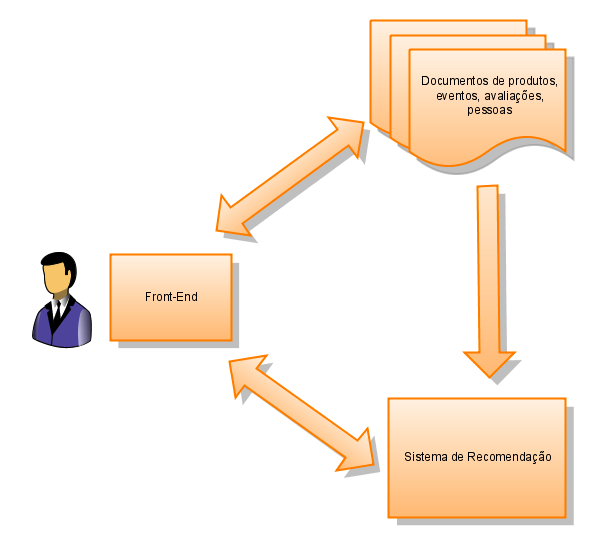
\includegraphics[width=\textwidth]{imagens/escopo}
  \caption{\it Diagrama de blocos do sistema}
  \label{fig:escopo}
\end{figure}

A Figura~\ref{fig:escopo} exibe o diagrama de blocos do sistema.

\subsubsection{Estrutura Analítca do Projeto} % (fold)
\label{ssub:estrutura_analítca_do_projeto}

\begin{itemize}

	\item Planejamento
		\subitem Definição do Escopo
			\subsubitem Examinar os objetivos do projeto
			\subsubitem Examinar os recursos necessários
			\subsubitem Elaborar o product backlog
		
	\item Pesquisa Bibliográfica
		\subitem Sistema de Recomendação
			\subsubitem Baseados em Conteúdo
			\subsubitem Filtragem Colaborativa
			\subsubitem Baseados em Confiança
		\subitem Web Semântica
			\subsubitem Microformatos
			\subsubitem Resource Description Framework (RDF)
			\subsubitem Web Ontology Language (OWL)
		\subitem Web Social
			\subsubitem Padrões de Projeto Sociais
	
	\item Conceituação
		\subitem Construir cenários e personas
		\subitem Selecionar as soluções possíveis e as funcionalidades necessárias
		\subitem Arquitetura da informação
		\subitem Avaliar a melhor solução
		
	\item Desenvolvimento
		\subitem Sistema de recomendação
			\subsubitem Captura e Parsing de documentos
			\subsubitem Algortimo de recomendação
			\subsubitem Interface de consulta de recomendações
		\subitem Base de documentos semânticos
		\subitem Front-End
			\subsubitem Aplicação para rede social
			\subsubitem Camada de Apresentação
			\subsubitem Integração com a base de documentos
			\subsubitem Integração com o Sistema de recomendação

\end{itemize}


% subsubsection estrutura_analítca_do_projeto (end)

\section{Motivação} % Apresentar a motivação e justificativa para a realização do trabalho (por exemplo, sua aplicabilidade prática, comparação com alternativas já existentes, potencial de aprendizado e evolução, etc).

 Recomendações sugerem itens para as pessoas ao invés de esperar que estes sejam descobertos passivamente. Ao oferecer valor aos usuários, fazendo suposições pertinentes sobre o tipo de objetos em que estão interessados, é possível conquistar a confiança deles. A vantagem para os usuários é a facilidade de encontrar a informação sem a ter a árdua tarefa de procurala.

 As plataformas sociais online têm modificado a forma com que as empresas utilizam a comunicação para o comércio. Pessoas estão utilizando a Internet para encontrar outras pessoas com interesses similares, fazer compras de forma mais eficiente, aprender sobre produtos e serviços e reclamar sobre produtos malfeitos e serviços pobres\cite{marketing_social_web}.

 A internet está rapidamente se tornando a mídia mais importante para o marketing. Os primeiros publicitários a utilizarem esse meio, que enxergaram essa mídia apenas como outro canal, não aproveitaram a melhor forma de fazer marketing na internet. A tendência é que as pessoas, cada vez mais bloqueiem os anúncios indesejados e queiram ter a capacidade de encontrar os produtos relevantes no momento adequado. É nesse contexto que surge a necessidade de uma plataforma que facilite a colaboração e que permita a criação e classificação de conteúdo pelos consumidores, de forma a permitir uma escolha mais inteligente dos melhores produtos e serviços e ao mesmo tempo criando uma mecanismo de feedback para as empresas interessadas.

 Devido à grande variedade atual de produtos e serviços, as pessoas têm cada vez mais dificuldade nas suas escolhas e na argumentação sobre a possível decisão. Quanto mais produtos similares de fabricantes diferentes ou serviços realizados por diversos prestadores, mais as pessoas se vêem desnorteadas e sem saber se a decisão realizada foi a mais correta. O mesmo ocorre com as empresas na hora de lançar os seus produtos. Os seus clientes pedem cada vez mais inovações e não há como saber a opinião de cada pessoa ou de um determinado grupo de pessoas sobre as novas características agregadas a um produto já lançado ou sobre novos produtos que agregarão tais inovações tecnológicas. Se a empresa tivesse posse dessas informações, ela também poderia decidir sobre o seu melhor caminho, ou seja, em quais tecnologias ou tipos de serviço investir.

 O projeto visa ter como resultado um produto que auxilia o processo de escolha com base na opinião das pessoas diretamente envolvidas. O sistema pretende organizar as opiniões de todos e deixar transparecer a opinião alheia, dessa forma as opiniões registradas podem ser capturadas pela comunidade.

\section{Alterações no Escopo do Projeto}

 Inicialmente o escopo do projeto englobava a criação de uma rede social utilizada para recomendações de bares e restaurantes. Os usuários procuravam estabelecimentos cadastrados na rede e conseguiam informações sobre os serviços prestados de acordo com notas e comentários feitos por outros usuários. Com isso, eles podiam recomendar bares e restaurantes para outros usuários.

 Também dentro do escopo estavam definidos os donos dos estabelecimentos que podiam tomar o cadastro próprio e gerenciá-lo para obter as informações estatísticas de quais tipos de pessoas haviam frequentado o seu bar ou restaurante. Com isso, formava-se um canal de comunicação com o cliente que consistia na resposta a perguntas feitas diretamente ao estabelecimento, além de divulgação de informações e novidades sobre o seu negócio.

 A segunda alteração no escopo do projeto tinha como objetivo a criação de uma ferramenta de groupware para que os usuários que utilizavam a rede pudessem marcar encontros e reuniões nos bares e restaurantes cadastrados. Groupware é um software colaborativo que apóia o trabalho em grupo. Nesse sistema o usuário poderia propor aos seus amigos um encontro em um determinado estabelecimento, sendo que os convidados poderiam aceitar ir ou não ao evento na data e horário estipulados.

 Por fim, a terceira modificação no escopo do projeto direciona a um objetivo próximo ao incialmente proposto. Após esta última alteração, o foco do projeto tornou-se o sistema de recomendação. Este sistema será alimentado com informações obtidas através de documentos semanticamente estruturados que descrevem produtos, eventos, avaliações e pessoas. Além disso o sistema de recomendação poderá considerar outros fatores tais como: semelhanças nas avaliações feitas por usuários; e na confiança de um usuário em outro. Baseado nestas informações o sistema deve sugerir novos itens ao usuário, de tal forma que estes sejam relevantes e confiáveis.

\subsection{Aplicações do Produto}
 
 O sistema pode ser aplicado para sugestão de qualquer item ao usuário, independentemente do conteúdo. No entanto, para permitir um experiência mais rica ao usuário as sugestões estarão restritas a documentos semanticamente estruturados. Estes documentos podem representar produtos, empresas, eventos, pessoas, lugares, websites e urls.
 
 Agregando o comportamento de vários usuários é possível identificar tendências e gerar recomendações baseadas nelas. Outra maneira de pensar nisto é que o sistema procura usuários que se comportam de maneira parecida quando estão escutando músicas, vendo filmes, ou lendo notícias.
 
 As relações de confiança entre usuários expressas através da Internet permitem que o sistema fornceça informações mais confiáveis para o usuário. Dessa forma, evita-se o uso do sistema para manipulação indevida.

 As recomendações geradas podem causar a serendipidade, ou seja, descobertas afortunadas de itens antes desconhecidos pelo usuário. Dessa forma, o usuário é capaz de econtrar uma informação de qualidade sem mesmo precisar procurala.

 Com base nas característas descritas acima, o sistema é adequado para servir de como ferramenta de apoio ao usuário em sistemas de e-commerce, através da sugestão de produtos, serviços e eventos nos quais o usuário pode vir a se interessar.